%!TEX encoding = UTF-8 Unicode
\documentclass{reqenglecture}

\title{Introduction to Software Requirements Engineering}

\subtitle{Part II: Functionality}

\author{Björn Regnell}

\date{\vspace{1em}\footnotesize Updated: \today~
\\ License: CC-BY-SA 
\\ \url{https://github.com/bjornregnell/reqeng-book} 
}

%\beamerdefaultoverlayspecification{<+->} %de-comment if you want pause after items

\begin{document}
\maketitle

\begin{frame}
\frametitle{Part II: Functionality}
\framesubtitle{Outline}
\tableofcontents
\end{frame}


\LectureOnly{\section{Modeling}}

\begin{Slide}{Requirements Modeling}

A requirements model...

\begin{itemize}
\item  is an informative \textbf{representation} of the intended system.

\item is an \textbf{abstraction} of the intended system 
\begin{itemize}
\item only \textit{some} aspects are represented, 
\item while other aspects are \textit{excluded}.

\end{itemize}
\item captures important knowledge gained from \textbf{elicitation}.

\item is often textual or a diagram, or both.

\item is often part of a \textbf{specification}.

\item should be \textbf{validated} by (some) stakeholders.

\end{itemize}
\end{Slide}

\begin{Slide}{Different aspects of requirements to model }

\begin{minipage}[t]{0.6\textwidth}
\begin{itemize}
\item Functional aspects:
\begin{itemize}
\item Data aspects:
\begin{itemize}
\item What is stored and processed by the system?
\item What is the format of input and output data?

\end{itemize}
\item Business Logic aspects: 
\begin{itemize}
\item How should the system behave in different usage contexts?
\item What output should be produced, given input and state?  
\end{itemize}
\end{itemize}
\end{itemize}
\end{minipage}%
\begin{minipage}[t]{0.4\textwidth}
\vspace{0.0em}\hfill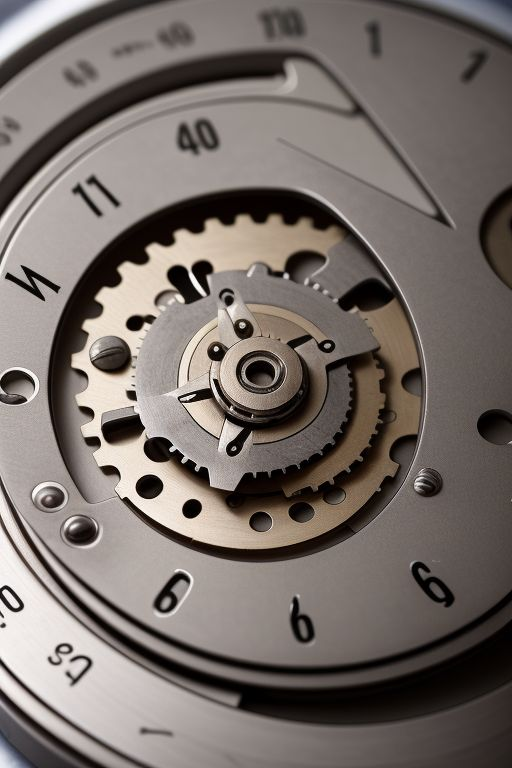
\includegraphics[width=0.82\textwidth]{../img/cog1}
\end{minipage}%

\begin{itemize}
\item Quality aspects: 
\begin{itemize}
\item What is a 'good' function from stakeholders' viewpoints?
\item More on quality modeling in Part III.

\end{itemize}
\end{itemize}
\end{Slide}

\begin{Slide}{Which modeling technique is best? }

\begin{itemize}
\item A modeling technique may be more or less suitable for representing some aspects of requirements from some stakeholders' viewpoint.

\item A \textbf{well-balanced combination} of modeling techniques can capture a more aspects in a better way than a single technique.

\item What modeling technique is best depends on...
\begin{itemize}
\item abstraction level
\item project type
\item stakeholders
\item tool support
\item the number and kind of requirements
\item ...

\end{itemize}
\item Model interpretation often requires specific knowledge: 
\begin{itemize}
\item Choose modeling technique based on stakeholders' ability to understand and validate!

\end{itemize}
\item How do you know that your chosen mix of models fit together and does not contradict each other?
\begin{itemize}
\item Make sure to check model inter-consistency in validation!

\end{itemize}
\end{itemize}
\end{Slide}
\begin{Slide}{Abstraction and level of detail}

\begin{minipage}[t]{0.4\textwidth}
\vspace{-1.0em}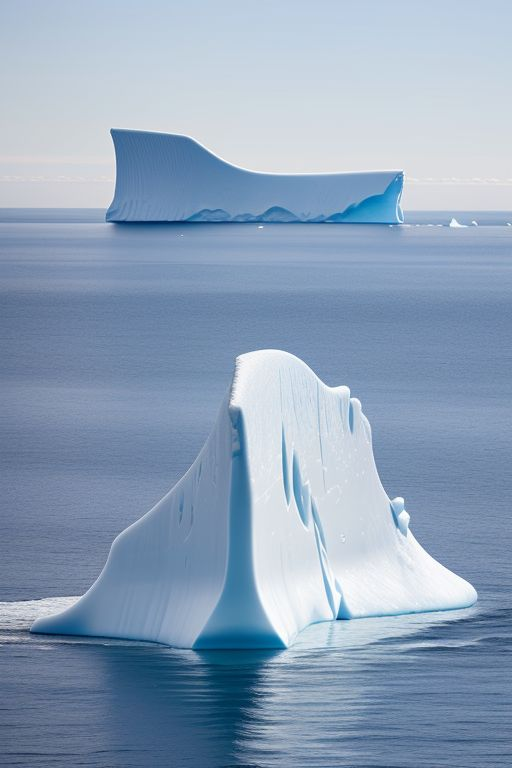
\includegraphics[width=1.0\textwidth]{../img/iceberg4}
\end{minipage}%
\begin{minipage}[t]{0.6\textwidth}
\begin{itemize}
\item The iceberg metaphor: 
\begin{itemize}
\item A req spec is only the tip of a massive iceberg of information
\end{itemize}
\item Abstraction means simplification
\begin{itemize}
\item focusing on what's important 
\item reduction of less relevant details
\end{itemize}
\item Different parts of the req space need different levels of detail
\end{itemize}
\end{minipage}%

\end{Slide}

\begin{Slide}{Mixed levels of detail over time}

\begin{itemize}
\item The picture below illustrates elaboration of reqs over time:
\begin{itemize}
\item Time on x-axis. Different reqs on y-axis. 
\item Lighter color means more elaboration.

\end{itemize}
\end{itemize}
\begin{minipage}[t]{1.0\textwidth}
\vspace{-1.0em}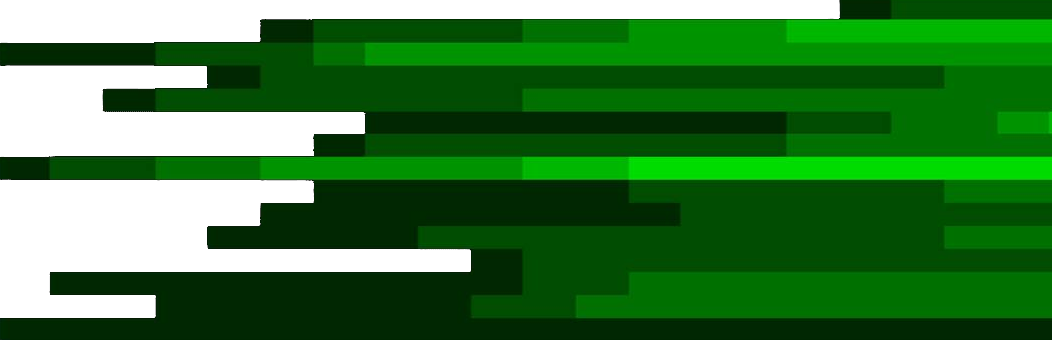
\includegraphics[width=1.0\textwidth]{../img/details-time}
\end{minipage}


\begin{itemize}
\item It is not cost-effective to spend the same amount of effort on all requirements.

\item Some requirements need more effort than others in elicitation, specification, validation and selection.




\end{itemize}
\end{Slide}
\begin{Slide}{Ontology}
\begin{itemize}
\item Ontology is the philosophical study of being:
\begin{itemize}
\item What types of entities exist?
\item How are entities grouped into categories? 
\item How are entities related to one another?
\end{itemize}
\item Example of ontological concepts
\begin{itemize}
\item Particulars and universals
\item Abstract and concrete
\item Identity and persistence over time
\item Modality: what is possible, actual, necessary?
\item Properties and relations
\end{itemize}
\item Further reading: 
\begin{itemize}
\item \url{https://en.wikipedia.org/wiki/Ontology}
\item \url{https://en.wikipedia.org/wiki/Ontology_engineering}

\end{itemize}
\end{itemize}
\end{Slide}
\LectureOnly{\section{Data}}
\begin{Slide}{Data Modeling }
\begin{itemize}
\item \textbf{Data dictionary}:  
\begin{itemize}
\item a list of data entities (classes) with textual descriptions of data attributes (fields) and relations among entities.
\end{itemize}
\item \textbf{Data views}: (a.k.a ''virtual windows'')
\begin{itemize}
\item examples of data values (instances) shown in a specific usage context sketched as a mockup screen
\item \textit{not} intended as interface design -- instead the focus is on modeling of stored and processed data 
\end{itemize}
\item \textbf{Data diagrams}: 
\begin{itemize}
\item boxes and arrows with data entities (classes), attributes (fields) and relations
\item \textbf{E/R-diagram}: focus on entities and their relations 
\item \textbf{Class diagram}: also inheritance, aggregation, methods
\end{itemize}
\item \textbf{Data format specifications}:
\begin{itemize}
\item Reqular expressions (regexp)
\item Protocol buffers (protobuf)

\end{itemize}
\end{itemize}
\end{Slide}
\begin{Slide}{Data dictionary example}
Parts of a data dictionary for a music streaming app:
\begin{Code}[language=reqt]
* Class: listener has
  * Spec: A user that listens to music.
  * Field: id has
    * Spec: A unique identifier of listener. Must not contain whitespace.
    * Example: abc.edf123
  * Field: password has
    * Spec: ...
* Class: artist has
  * Spec: ...
* Class: track has
  * Spec: ...
* Class: album has
  * Spec: ...
\end{Code}
Each data entity (class) together with attributes (fields) are specified in natural language.
\end{Slide}

\begin{Slide}{Data Views}
\begin{minipage}[t]{0.55\textwidth}
\begin{itemize}
\item Example data shown in a mockup screen.
\item Good for data model validation with stakeholders.
\begin{itemize}
\item Are examples relevant?
\item Any missing data?
\end{itemize}
\item Also called ''virtual window''.
\item Not a user interface design.
\end{itemize}
\end{minipage}%
\begin{minipage}[t]{0.45\textwidth}
\vspace{-1.0em}\hfill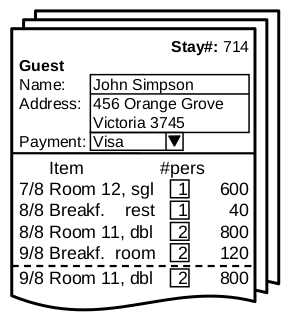
\includegraphics[width=0.85\textwidth]{../img/virtual-window}

{\hfill\fontsize{4}{4}\fontfamily{qtm}\itshape\selectfont From: S. Lauesen ''Software Requirements'' \textcopyright~Addison-Wesley 2002}

\end{minipage}
\end{Slide}

\begin{Slide}{Entity-Relationship-diagram}
\footnotesize\url{https://en.wikipedia.org/wiki/Entity-relationship_model}

\begin{minipage}[t]{0.9\textwidth}
\vspace{-0.4em}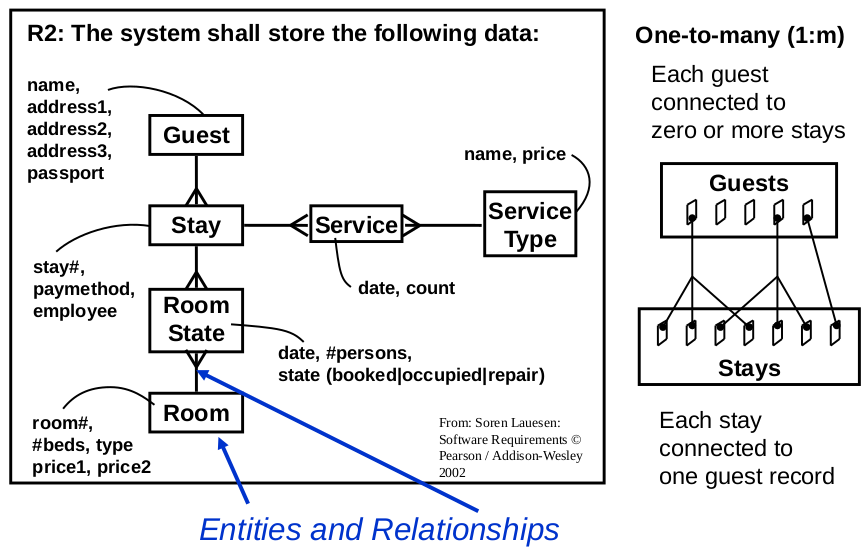
\includegraphics[width=1.0\textwidth]{../img/ER-diagram}
\vspace{-0.1em}
\end{minipage}

{\hfill\fontsize{5}{5}\fontfamily{qtm}\itshape\selectfont From: S. Lauesen ''Software Requirements'' \textcopyright~Addison-Wesley 2002}
\end{Slide}

\begin{Slide}{Class diagram}
\footnotesize\url{https://en.wikipedia.org/wiki/Class_diagram}

\begin{minipage}[t]{0.82\textwidth}
\vspace{-0.4em}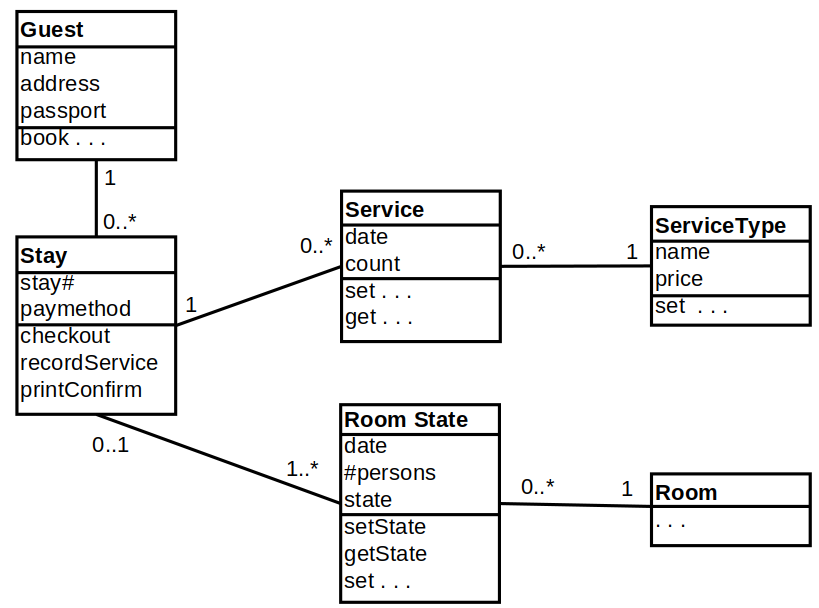
\includegraphics[width=1.0\textwidth]{../img/uml-class-diagram}
\vspace{-1.4em}
\end{minipage}

{\hfill\fontsize{5}{5}\fontfamily{qtm}\itshape\selectfont From: S. Lauesen ''Software Requirements'' \textcopyright~Addison-Wesley 2002}



\end{Slide}

\LectureOnly{\section{Logic}}
\begin{Slide}{Business Logic Modeling}
\begin{itemize}
\item Functional modeling techniques with focus on \textbf{logic}:
\begin{itemize}
\item sadfadsf

\end{itemize}
\end{itemize}
\end{Slide}
\begin{Slide}{Work Split: When to decide who does what?}

\begin{itemize}
\item Domain-focused logic: 
\begin{itemize}
\item users' work and system behaviour is joint
\item the work split is decided in later design
\end{itemize}
\item Product-focused logic: 
\begin{itemize}
\item users' work and system behaviour is separated  
\item the work split is explicitly specified in req spec
 

\end{itemize}
\end{itemize}
\end{Slide}
\LectureOnly{\section{Usage}}
\begin{Slide}{Contextual usage modeling}
Also called \textbf{scenario-based requirements} 
{\footnotesize\url{https://en.wikipedia.org/wiki/Scenario_(computing)}}
\begin{itemize}
\item User story:
\begin{itemize}
\item Short description of what a user role wants to do with the system in order to achieve a goal.
\item {\footnotesize\url{https://en.wikipedia.org/wiki/User_story}}
\end{itemize}
\item Use cases and tasks: 
\begin{itemize}
\item \textit{Domain-focus:} often called (user) \textbf{task}\\
    A piece of work by users, potentially supported by a system.
\item \textit{Product-focus:} often called \textbf{use case}\\
    A goal-fulfilling interaction between users and the product.
\item {\footnotesize\url{https://en.wikipedia.org/wiki/Use_case}}
\end{itemize}
\item Narrative:
\begin{itemize}
\item A detailed story from a user's perspective including thoughts and emotions when using the system for a specific purpose.



\end{itemize}
\end{itemize}
\end{Slide}
\begin{Slide}{User Stories}
\begin{itemize}
\item Short description of what a user role wants to do with the system in order to achieve a goal. 
\item Some proposed templates:
\begin{itemize}
\item \fontsize{9}{11}\selectfont\code{As a <role> I can <capability>, so that <receive benefit>.}
\item \fontsize{9}{11}\selectfont\code{In order to <receive benefit> as a <role>, I can <desire>.}
\item \fontsize{9}{11}\selectfont\code{As <who> <when> <where>, I want <what> because <why>.}


\end{itemize}
\end{itemize}
\end{Slide}
\begin{Slide}{Use cases}
\begin{itemize}
\item Definition according to \url{https://en.wikipedia.org/wiki/Use_case}
\begin{itemize}
\item  A usage scenario for a piece of software.
\item  A potential scenario in which a system receives an external request and responds to it.

\end{itemize}
\end{itemize}
\vspace{-0.5em}
\begin{minipage}[t]{0.55\textwidth}
\begin{itemize}
\item Contents of textual use case:
\begin{itemize}
\item Title
\item Primary Actor
\item Brief (corresponds to user story)
\item Stakeholders
\item Pre- and postconditions
\item Triggers
\item Basic flows
\item Extensions
\end{itemize}
\end{itemize}
\end{minipage}%
\hfill\begin{minipage}[t]{0.45\textwidth}
\vspace{-0.4em}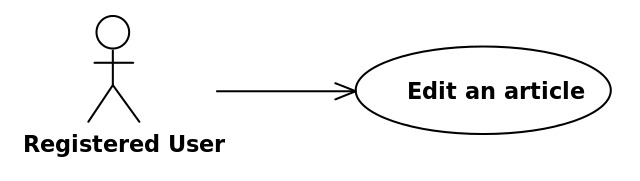
\includegraphics[width=1.0\textwidth]{../img/use-case-edit-article}
\end{minipage}
\end{Slide}

\begin{Slide}{Narratives and personas}

\begin{itemize}
\item \footnotesize\url{https://en.wikipedia.org/wiki/Scenario_(computing)}
\item \url{https://en.wikipedia.org/wiki/Persona_(user_experience)}

\end{itemize}
\begin{minipage}[t]{0.85\textwidth}
\vspace{-0.4em}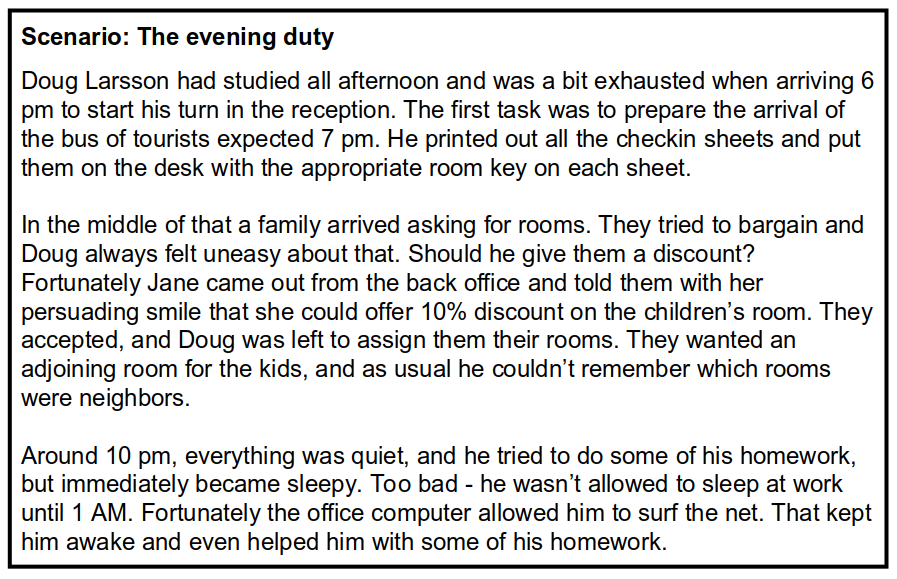
\includegraphics[width=1.0\textwidth]{../img/vivid-scenario}
\vspace{-1.0em}
\end{minipage}

{\fontsize{5}{5}\fontfamily{qtm}\itshape\selectfont From: S. Lauesen ''Software Requirements'' \textcopyright~Addison-Wesley 2002}

\end{Slide}

\LectureOnly{\section{Behavior}}
\begin{Slide}{System behavior modeling}

\begin{itemize}
\item State Machines

\item Interaction Diagrams

\item Data Flow Diagrams


\end{itemize}
\end{Slide}
\begin{Slide}{State diagram example}
\begin{minipage}[t]{0.65\textwidth}
\vspace{0.4em}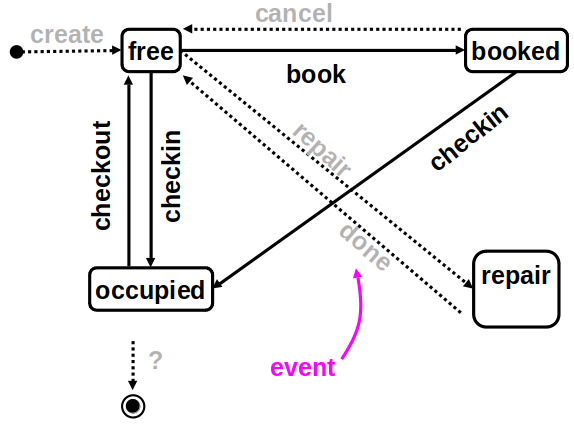
\includegraphics[width=1.0\textwidth]{../img/state-diagram}
\vspace{-0.4em}
\end{minipage}

{\vspace*{1em}\fontsize{5}{5}\fontfamily{qtm}\itshape\selectfont From: S. Lauesen ''Software Requirements'' \textcopyright~Addison-Wesley 2002}
\end{Slide}

\begin{Slide}{Sequence Diagrams}
\begin{itemize}
\item ...

\end{itemize}
\end{Slide}
\begin{Slide}{Data-flow diagram example}
\begin{minipage}[t]{0.6\textwidth}
\vspace{0.4em}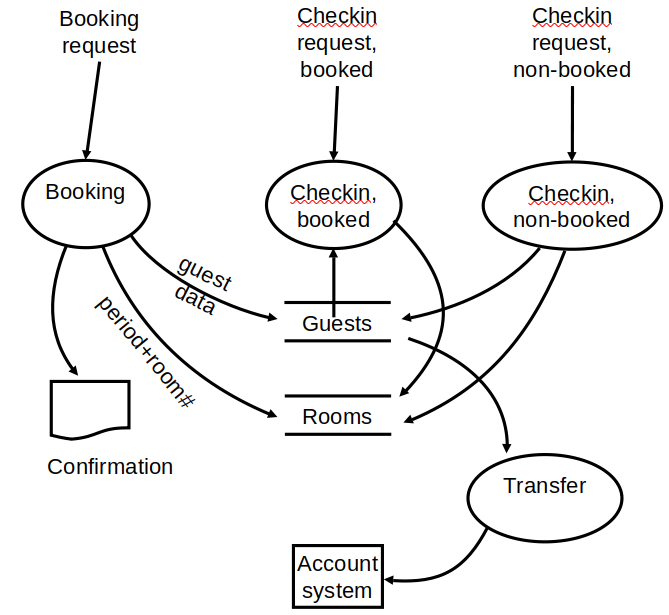
\includegraphics[width=1.0\textwidth]{../img/data-flow-diagram}
\vspace{-1.4em}
\end{minipage}%
\hfill\begin{minipage}[t]{0.3\textwidth}
\vspace{-0.1em}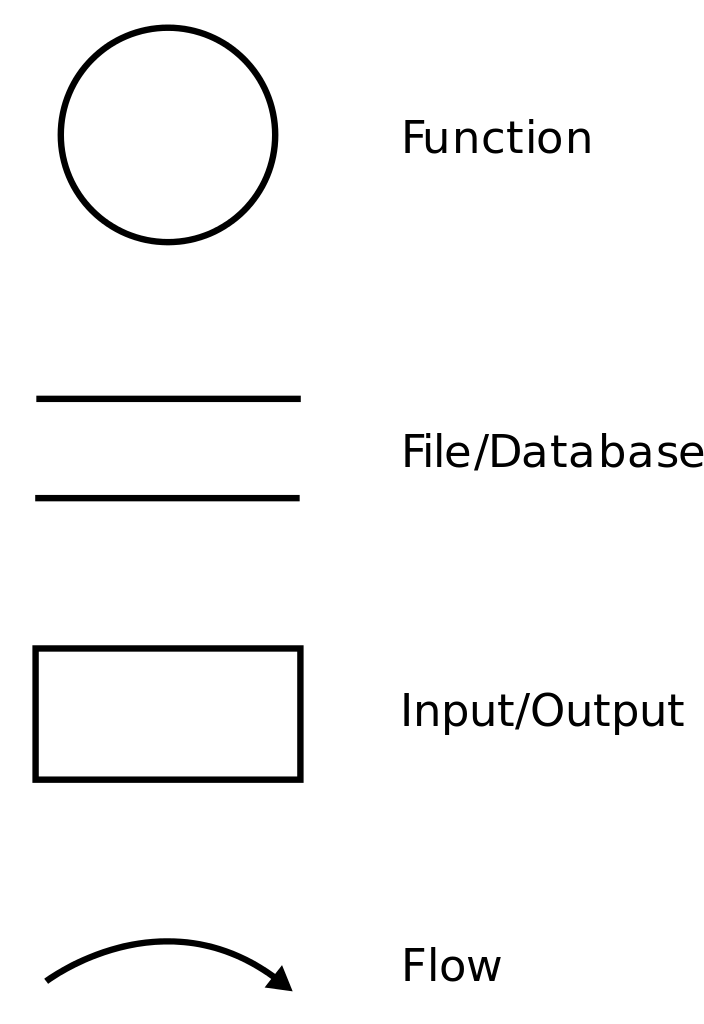
\includegraphics[width=0.8\textwidth]{../img/data-flow-diagram-symbols}
\end{minipage}%

{\vspace*{1em}\fontsize{5}{5}\fontfamily{qtm}\itshape\selectfont From: S. Lauesen ''Software Requirements'' \textcopyright~Addison-Wesley 2002}
\end{Slide}

\LectureOnly{\section{Prototyping}}
\begin{Slide}{What is prototyping?}
\begin{itemize}
\item Prototyping is a creative practice within product design.
\item A prototype can range from 
\begin{itemize}
\item a simple paper \textbf{sketch}, through 
\item a computer-generated \textbf{mock-up}, to an 
\item incomplete version of the production software
\end{itemize}
\item Aspects of a prototype:
\begin{itemize}
\item Purpose 
\item Scope 
\item Media 
\item Usage 

\end{itemize}
\end{itemize}
\end{Slide}
\begin{Slide}{Prototype Scoping}

\begin{itemize}
\item Breadth of functionality
\item Functional refinement:
\begin{itemize}
\item Visual appearance
\item Interactive and haptic behavior
\item Data realism

\end{itemize}
\end{itemize}
\end{Slide}
\begin{Slide}{Prototyp Media}
\begin{itemize}
\item TODO
\begin{itemize}
\item ...


\end{itemize}
\end{itemize}
\end{Slide}
\begin{Slide}{Prototype Usage}
\begin{itemize}
\item Reviewers 
\begin{itemize}
\item internal
\item with families, friends and foes
\item external
\end{itemize}
\item Prototype interaction 
\begin{itemize}
\item yes 
\item no (demo)
\end{itemize}
\item Review approach
\begin{itemize}
\item scenario-based
\item free
\end{itemize}
\item Usage environment
\begin{itemize}
\item \textit{in vitro}: lab setting, different from final product usage 
\item \textit{in vivo}: real world setting, similar to final product usage

\end{itemize}
\end{itemize}
\end{Slide}
\begin{Slide}{Exploration Strategy}
\begin{itemize}
\item TODO
\begin{itemize}
\item ...

\end{itemize}
\end{itemize}
\end{Slide}
\LectureOnly{\section{Delegation}}
\begin{Slide}{Delegated Requirements}
\begin{itemize}
\item What?
\begin{itemize}
\item ...
\end{itemize}
\item Why?
\begin{itemize}
\item ...

\end{itemize}
\end{itemize}
\end{Slide}
\begin{Slide}{Standards as requirements}
\begin{itemize}
\item What?
\begin{itemize}
\item ...
\end{itemize}
\item Why?
\begin{itemize}
\item ...


\end{itemize}
\end{itemize}
\end{Slide}
\begin{Slide}{Regulatory requirements}
\begin{itemize}
\item What?
\begin{itemize}
\item ...
\end{itemize}
\item Why?
\begin{itemize}
\item ...

\end{itemize}
\end{itemize}
\end{Slide}
\begin{Slide}{Test cases as requirements}
\begin{itemize}
\item What?
\begin{itemize}
\item ...
\end{itemize}
\item Why?
\begin{itemize}
\item ...

\end{itemize}
\end{itemize}
\end{Slide}
\begin{Slide}{Development process requirements}
\begin{itemize}
\item What?
\begin{itemize}
\item ...
\end{itemize}
\item Why?
\begin{itemize}
\item ...

\end{itemize}
\end{itemize}
\end{Slide}
\end{document}